\section{ساختار و عملکرد فیزیکی \lr{MOS}}
\label{sec:book-mos-structure}
\subsection{\lr{Silicon}، \lr{Dopant} و حامل متحرک}
اتم \lr{Silicon} چهار الکترون ظرفیت دارد و در شبکه بلوری با همسایه‌ها پیوند
تشکیل می‌دهد. هدایت الکتریکی به وجود حامل‌های متحرک وابسته است.
در دمای غیرصفر، \lr{Silicon} خالص نیز می‌تواند الکترون و \lr{Hole} ناشی از
برانگیزش گرمایی داشته باشد. افزودن مقدار کنترل‌شده ناخالصی، یا \lr{Doping}،
تعداد و نوع حامل غالب را تغییر می‌دهد. اسلایدهای ۲ و ۳ این مقدمه را به صورت
تصویر شبکه و ناخالصی نشان می‌دهند \cite{mos}.

در \lr{n-type}، ناخالصی \lr{Donor} از گروه پنج، مانند \lr{Arsenic}، یک الکترون
اضافی در اختیار هدایت می‌گذارد. پس از آزادشدن الکترون، یون ناخالصی مثبت در شبکه
باقی می‌ماند. در \lr{p-type}، ناخالصی \lr{Acceptor} از گروه سه، مانند
\lr{Boron}، کمبود الکترونی ایجاد می‌کند که به صورت \lr{Hole} توصیف می‌شود.
حرکت پی‌درپی الکترون‌های پیوندی برای پرکردن این جای خالی، مانند جابه‌جایی
حاملی با بار مثبت دیده می‌شود. یون‌های ناخالصی در شبکه ثابت‌اند، اما حامل‌ها متحرک‌اند.

در \lr{n-type}، الکترون‌ها و در \lr{p-type}، \lr{Hole}ها حامل غالب‌اند.
\lr{Doping} معمولاً ماده را در مقیاس حجمی تقریباً خنثی نگه می‌دارد، زیرا بار
حامل‌های متحرک و یون‌ها یکدیگر را جبران می‌کنند. در ناحیه \lr{Depletion}،
خارج‌شدن حامل‌های متحرک، بار یون‌های ثابت را آشکار می‌کند.
این توضیح، معنای دقیق‌تر تقریب «نبود حامل آزاد» در مدل مقدماتی اسلاید ۳ و
متن ساده‌شده صفحه ۶۲ کتاب را فراهم می‌کند.

\subsection{پیوند \lr{p-n} و اتصال \lr{Body}}
تماس ناحیه \lr{p-type} و \lr{n-type} یک پیوند \lr{p-n} می‌سازد.
در مدل دیودی، سمت \lr{p}، \lr{Anode} و سمت \lr{n}، \lr{Cathode} است.
وقتی ولتاژ سمت \lr{p} نسبت به سمت \lr{n} افزایش کافی داشته باشد، پیوند
\lr{Forward-biased} می‌شود. با منفی‌ترشدن سمت \lr{p} نسبت به سمت \lr{n}،
پیوند \lr{Reverse-biased} است و جریان نشتی کوچکی دارد. این مدل مقدماتی
در اسلاید ۴ معرفی شده است \cite{mos}.

در \lr{nMOS}، دو ناحیه \(n^+\) داخل \lr{Body} نوع \lr{p} قرار دارند.
هر یک با \lr{Body} پیوند دیودی دارد. با اتصال \lr{Body} به زمین و ولتاژهای
نامنفی \lr{Source} و \lr{Drain}، این پیوندها بایاس صفر یا معکوس دارند.
در \lr{pMOS}، ناحیه‌های \(p^+\) داخل \lr{Body} نوع \lr{n} هستند و معمولاً
\lr{Body} به بالاترین تغذیه وصل می‌شود. این اتصال پیوندها را در شرایط معمول
مدار از هدایت مستقیم دور نگه می‌دارد \cite[صفحات ۶۲ تا ۶۴]{weste}.

علامت \(+\) در \(n^+\) یا \(p^+\) بیانگر شدت بیشتر \lr{Doping} است.
در ساختمان \lr{MOS}، مسیر کنترل‌شده جریان از لایه زیر \lr{Gate} عبور می‌کند.
بایاس ناخواسته پیوند \lr{Body} می‌تواند مسیر دیگری برای جریان ایجاد کند، بنابراین
پایانه چهارم در بررسی مدار اهمیت دارد.

\subsection{پشته \lr{MOS} و سه وضعیت سطح \lr{Silicon}}
نام کامل \lr{MOS}، عبارت \lr{Metal-Oxide-Semiconductor} است.
لایه \lr{Gate} رسانا، لایه میانی \lr{Gate Oxide} عایق و لایه زیرین نیمه‌رسانای
\lr{Body} است. کتاب به کاربرد تاریخی \lr{Metal Gate}، استفاده از
\lr{Polysilicon} و بازگشت \lr{Metal Gate} در فناوری‌های مورد بحث خود اشاره می‌کند
\cite[صفحه ۶۱]{weste}. عایق میان \lr{Gate} و سطح، امکان کنترل بار سطح با میدان
الکتریکی را فراهم می‌کند.

برای دیدن سه وضعیت سطح، ابتدا ساختار \lr{MOS Capacitor} با \lr{Body} نوع
\lr{p} و متصل به زمین را در نظر می‌گیریم. توصیف ساده کتاب، اثر اختلاف
\lr{Work Function} و بار ثابت اکسید را در نمودار مقدماتی کنار می‌گذارد.
در مدل دقیق، محل آغاز این وضعیت‌ها نسبت به صفر ولتاژ به \lr{Flat-band Voltage}
و پارامترهای ساخت وابسته است. شکل \ref{fig:mos-surface} سه حالت مقدماتی را نشان می‌دهد.

\begin{figure}[ht]
\centering
\begin{latin}
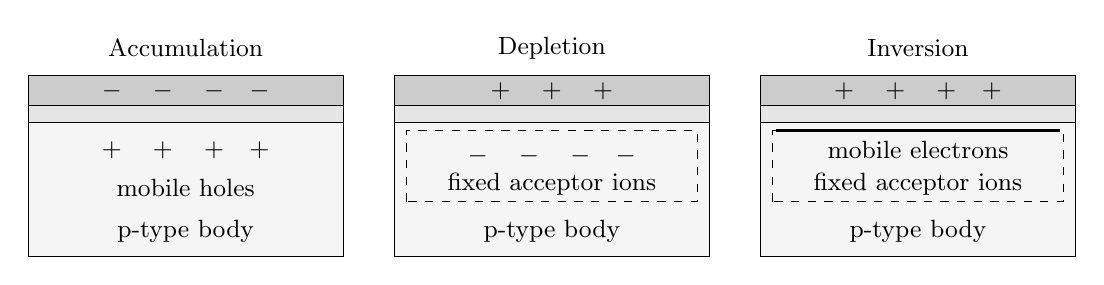
\begin{tikzpicture}[x=1cm,y=1cm,font=\small]
\foreach \x/\title in {0/Accumulation,4.65/Depletion,9.3/Inversion}{
 \draw[fill=gray!8] (\x,0) rectangle +(4,1.7);
 \draw[fill=gray!20] (\x,1.7) rectangle +(4,0.22);
 \draw[fill=gray!40] (\x,1.92) rectangle +(4,0.38);
 \node at (\x+2,2.65) {\title};
 \node at (\x+2,0.32) {p-type body};
}
\node at (2,2.1) {$-\quad-\quad-\quad-$};
\node at (2,1.35) {$+\quad+\quad+\quad+$};
\node at (2,0.87) {mobile holes};
\node at (6.65,2.1) {$+\quad+\quad+$};
\draw[dashed] (4.8,0.7) rectangle (8.5,1.6);
\node at (6.65,1.28) {$-\quad-\quad-\quad-$};
\node at (6.65,0.92) {fixed acceptor ions};
\node at (11.3,2.1) {$+\quad+\quad+\quad+$};
\draw[dashed] (9.45,0.7) rectangle (13.15,1.6);
\draw[very thick] (9.5,1.6)--(13.1,1.6);
\node at (11.3,1.36) {mobile electrons};
\node at (11.3,0.92) {fixed acceptor ions};
\end{tikzpicture}
\end{latin}
\caption{بازنمایی آموزشی سه وضعیت سطح \lr{MOS Capacitor} بر پایه شکل
\secnum{۲.۲} کتاب و اسلاید ۹. نوار میانی نازک، اکسید و نوار بالایی، \lr{Gate} است.
علامت‌های بار شماتیک‌اند و تعداد واقعی حامل‌ها را نشان نمی‌دهند \cite{weste,mos}.}
\label{fig:mos-surface}
\end{figure}

در \lr{Accumulation}، ولتاژ منفی \lr{Gate}، \lr{Hole}های مثبت را به سطح
جذب می‌کند. تراکم حامل غالب نزدیک سطح بیشتر می‌شود.
در \lr{Depletion}، ولتاژ مثبت کوچک \lr{Gate}، \lr{Hole}ها را از سطح دور
می‌کند و ناحیه‌ای با بار یون‌های منفی ثابت \lr{Acceptor} باقی می‌ماند.
در \lr{Inversion}، ولتاژ مثبت کافی، الکترون‌ها را به نزدیکی سطح می‌آورد و
لایه‌ای با حامل غالب الکترونی روی \lr{Body} نوع \lr{p} تشکیل می‌شود.
نوع حامل غالب در سطح تغییر می‌کند، درحالی‌که نوع \lr{Doping} کل \lr{Body} ثابت است.

\lr{Threshold Voltage} یا \(V_t\)، مرز قراردادی تشکیل \lr{Strong Inversion}
در این مدل است. مقدار آن به ساختار و \lr{Doping}، ضخامت اکسید و بایاس بستگی دارد.
در ترانزیستور \lr{Enhancement-mode nMOS} این درس، \(V_{tn}>0\) فرض می‌شود.
کتاب امکان مهندسی آستانه منفی را نیز یادآوری می‌کند.
در استخراج مقدماتی، \(V_t\) ثابت است و اثر بایاس \lr{Body} در بخش
\secnum{۲.۴} بررسی خواهد شد.

\subsection{پایانه‌ها، نمادها و جهت جریان}
چهار پایانه افزاره \lr{Gate}، \lr{Source}، \lr{Drain} و \lr{Body} هستند.
نماد سه‌پایانه اتصال \lr{Body} را به طور ضمنی نشان می‌دهد و در نماد چهارپایانه،
این اتصال آشکار است. کتاب در شکل \secnum{۲.۱} چند قرارداد رسم را نشان می‌دهد.
در نماد متداول اسلایدها، حباب روی \lr{Gate} رفتار معکوس \lr{pMOS} را مشخص می‌کند.
هنگام خواندن شکل، نوع افزاره و اتصال \lr{Body} را هم‌زمان بررسی می‌کنیم
\cite[صفحه ۶۱]{weste}.

هر ولتاژ دوپایانه‌ای، اختلاف پتانسیل پایانه اول و دوم است. تعریف‌ها چنین‌اند
\begin{equation}
 V_{GS}=V_G-V_S,\qquad V_{GD}=V_G-V_D,\qquad
 V_{DS}=V_D-V_S.
 \label{eq:mos-terminal-voltages}
\end{equation}
با کم‌کردن دو ولتاژ اول، \(V_G\) حذف می‌شود و داریم
\begin{equation*}
 V_{GS}-V_{GD}=(V_G-V_S)-(V_G-V_D)=V_D-V_S=V_{DS}.
\end{equation*}
این رابطه همان اسلاید ۱۰ است. برابرگرفتن \(V_{GS}\) با \(V_G\) هنگامی معتبر است
که \(V_S=0\) باشد.

در مدل متقارن مورد استفاده، برای \lr{nMOS} پایانه کم‌پتانسیل‌تر را
\lr{Source} می‌گیریم تا \(V_{DS}\ge0\) باشد. الکترون‌ها از \lr{Source} به
\lr{Drain} حرکت می‌کنند. به دلیل بار منفی الکترون، جریان قراردادی مثبت
\(I_{DS}\) از \lr{Drain} به \lr{Source} است. در \lr{pMOS}،
\lr{Source} پایانه پرپتانسیل‌تر و حرکت \lr{Hole} و جریان قراردادی از
\lr{Source} به \lr{Drain} است \cite[صفحه ۶۴]{weste}.

\subsection{تشخیص \lr{Cutoff}، \lr{Linear} و \lr{Saturation}}
برای \lr{nMOS} با \(V_{tn}>0\)، اگر \(V_{GS}<V_{tn}\) باشد، کانال
\lr{Strong Inversion} تشکیل نمی‌شود و افزاره در \lr{Cutoff} است.
مدل مرتبه اول جریان را صفر می‌گیرد. نشتی واقعی در بخش \secnum{۲.۴} بررسی می‌شود.
وقتی \(V_{GS}>V_{tn}\)، سمت \lr{Source} کانال تشکیل می‌شود.
اگر \(V_{DS}=0\)، با وجود کانال، اختلاف پتانسیل طولی و جریان خالص صفر است
\cite[شکل \secnum{۲.۳}]{weste}.

برای ولتاژ \lr{Drain} مثبت کوچک، کانال تا سمت \lr{Drain} ادامه دارد.
شرط تشکیل کانال در آن سمت \(V_{GD}>V_{tn}\) است.
با جای‌گذاری \(V_{GD}=V_{GS}-V_{DS}\)، این شرط به
\begin{equation}
 V_{DS}<V_{GS}-V_{tn}
 \label{eq:mos-linear-condition}
\end{equation}
تبدیل می‌شود. نام‌های \lr{Linear}، \lr{Triode}، \lr{Resistive} و
\lr{Nonsaturated} در کتاب برای این ناحیه به کار رفته‌اند.
تناسب تقریباً خطی جریان با \(V_{DS}\) هنگامی دقیق‌تر است که \(V_{DS}\) خیلی
کوچک‌تر از \(V_{GS}-V_{tn}\) باشد.

در مرز \(V_{DS}=V_{GS}-V_{tn}\)، اضافه‌ولتاژ مؤثر انتهای کانال صفر می‌شود.
با افزایش بیشتر \(V_{DS}\)، کانال در نزدیکی \lr{Drain} دچار \lr{Pinch-off}
می‌شود. حامل‌ها از انتهای کانال به ناحیه میدان قوی رسیده و به \lr{Drain}
منتقل می‌شوند. جریان برقرار می‌ماند. در مدل \lr{Long-channel} ایدئال، مقدار آن
برای \(V_{GS}\) ثابت تقریباً مستقل از \(V_{DS}\) است. این ناحیه
\lr{Saturation} نام دارد \cite[صفحات ۶۳ و ۶۴]{weste}.

شکل \ref{fig:mos-channel-shape} کاهش بار موضعی کانال از سمت \lr{Source}
به \lr{Drain} را نمایش می‌دهد. ضخامت ترسیمی، بزرگی بار را به طور شماتیک نشان می‌دهد.
\begin{figure}[ht]
\centering
\begin{latin}
\PersianMathDigits
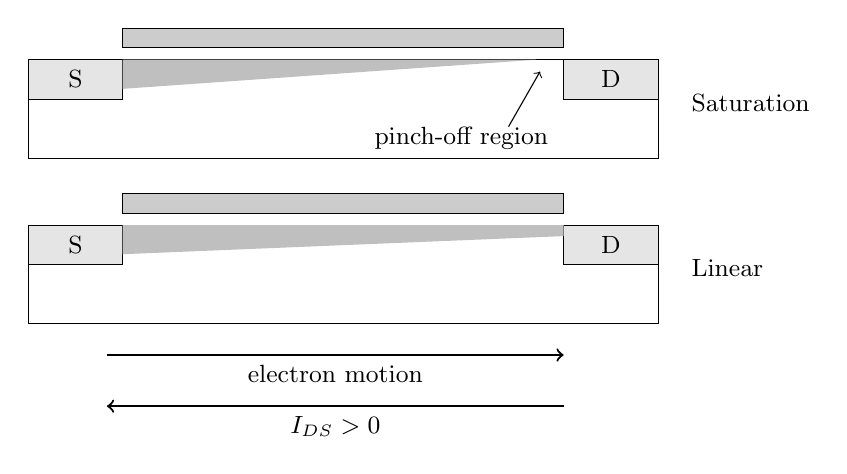
\begin{tikzpicture}[x=1cm,y=1cm,font=\small]
\foreach \y/\name in {0/Linear,2.1/Saturation}{
 \draw (0,\y) rectangle (8,\y+1.25);
 \draw[fill=gray!20] (0,\y+0.75) rectangle (1.2,\y+1.25);
 \draw[fill=gray!20] (6.8,\y+0.75) rectangle (8,\y+1.25);
 \draw[fill=gray!40] (1.2,\y+1.4) rectangle (6.8,\y+1.65);
 \draw (1.2,\y+1.25)--(6.8,\y+1.25);
 \node at (0.6,\y+1) {S};\node at (7.4,\y+1) {D};
 \node[anchor=west] at (8.3,\y+0.7) {\name};
}
\fill[gray!50] (1.2,1.25)--(6.8,1.25)--(6.8,1.11)--(1.2,0.88)--cycle;
\fill[gray!50] (1.2,3.35)--(6.45,3.35)--(1.2,2.98)--cycle;
\draw[->] (6.1,2.5)--(6.5,3.2);
\node at (5.5,2.35) {pinch-off region};
\draw[->,thick] (1,-0.4)--(6.8,-0.4) node[midway,below] {electron motion};
\draw[<-,thick] (1,-1.05)--(6.8,-1.05) node[midway,below] {$I_{DS}>0$};
\end{tikzpicture}
\end{latin}
\caption{نمای آموزشی کانال در دو ناحیه کاری، بر پایه شکل \secnum{۲.۳} کتاب.
کانال نزدیک \lr{Drain} بار کمتری دارد. در \lr{Saturation} حامل‌ها از ناحیه
\lr{Pinch-off} به \lr{Drain} انتقال می‌یابند \cite{weste}.}
\label{fig:mos-channel-shape}
\end{figure}

برای اختصار، \lr{Overdrive Voltage} را مطابق نماد کتاب به صورت
\(V_{GT}=V_{GS}-V_{tn}\) تعریف می‌کنیم. جدول \ref{tab:mos-regions} روند انتخاب
ناحیه را خلاصه می‌کند. در مدل قطعه‌ای، نقطه آستانه را با جریان صفر به
\lr{Cutoff} و مرز \lr{Linear} و \lr{Saturation} را به ناحیه دوم نسبت می‌دهیم.
دو رابطه جریان در مرز دوم یک مقدار می‌دهند.
\clearpage
\begin{table}[ht]
\centering
\caption{ناحیه‌های \lr{nMOS} با فرض \(V_{DS}\ge0\) و آستانه ثابت.}
\label{tab:mos-regions}
\begin{tabularx}{\textwidth}{rXX}
\toprule
ناحیه & شرط & تفسیر\\
\midrule
\lr{Cutoff} & \(V_{GS}\le V_{tn}\) & جریان صفر در مدل مرتبه اول\\
\lr{Linear} & \(V_{GS}>V_{tn},\ 0\le V_{DS}<V_{GT}\) & کانال تا دو انتها برقرار است\\
\lr{Saturation} & \(V_{GS}>V_{tn},\ V_{DS}\ge V_{GT}\) & جریان ایدئال با ولتاژ \lr{Gate} تعیین می‌شود\\
\bottomrule
\end{tabularx}
\end{table}

\subsection{مثال‌های تشخیص ناحیه با \lr{Source} غیرصفر}
در مثال‌های فرضی این قسمت، \(V_{tn}=\qty{0.4}{\volt}\) ثابت است.
اگر \(V_G=\qty{1.2}{\volt}\)، \(V_S=\qty{0.3}{\volt}\) و
\(V_D=\qty{0.5}{\volt}\) باشند، ابتدا اختلاف‌ها را حساب می‌کنیم
\[
 V_{GS}=1.2-0.3=\qty{0.9}{\volt},\qquad
 V_{DS}=0.5-0.3=\qty{0.2}{\volt},\qquad
 V_{GT}=0.9-0.4=\qty{0.5}{\volt}.
\]
چون \(V_{GS}>V_{tn}\) و \(0.2<0.5\)، ناحیه \lr{Linear} است.
از سوی دیگر \(V_{GD}=1.2-0.5=\qty{0.7}{\volt}>V_{tn}\) نیز همان نتیجه را تأیید می‌کند.

اگر تنها \(V_D\) به \qty{1.0}{\volt} تغییر کند، \(V_{DS}=\qty{0.7}{\volt}\)
و \(V_{GD}=\qty{0.2}{\volt}\) می‌شوند. شرط \(V_{DS}\ge V_{GT}\) برقرار است
و ترانزیستور در \lr{Saturation} قرار می‌گیرد. اگر در حالت دیگری
\(V_G=\qty{0.6}{\volt}\) باشد و \(V_S=\qty{0.3}{\volt}\) باقی بماند،
\(V_{GS}=\qty{0.3}{\volt}<V_{tn}\) و ترانزیستور در \lr{Cutoff} است.
شرط روشن‌شدن پیش از مقایسه \(V_{DS}\) با \(V_{GT}\) بررسی می‌شود.

برای \lr{Body} ثابت و \lr{Source} متحرک، آستانه واقعی می‌تواند با
\lr{Body Effect} تغییر کند. این سه مثال برای تمرین اختلاف ولتاژ، آستانه را
ثابت فرض کرده‌اند. تحلیل اثر بایاس \lr{Body} در دامنه بخش \secnum{۲.۴} است.
\subsection{ولتاژ تغذیه و محدودیت اکسید}
\(V_{DD}\) ولتاژ ریل تغذیه نسبت به \lr{GND} با مرجع صفر است.
اسلاید ۲۵، تغذیه \qty{5}{\volt} در مثال تاریخی دهه ۱۹۸۰ و کاهش ولتاژ در
فناوری‌های مورد بحث خود را نشان می‌دهد \cite{mos}.
با نازک‌شدن اکسید، همان اختلاف ولتاژ می‌تواند میدان عمودی بزرگ‌تری ایجاد کند.
در مدل یکنواخت، بزرگی میدان اکسید تقریباً \(E_{\mathrm{ox}}=V_{\mathrm{ox}}/t_{\mathrm{ox}}\)
است، که \(V_{\mathrm{ox}}\) ولتاژ دو سوی خود اکسید است.
انتخاب تغذیه باید با محدودیت افزاره و مشخصات فناوری سازگار باشد.
کاهش ولتاژ در رابطه توان دینامیکی، انرژی هر شارژ را کاهش می‌دهد.
هم‌زمان، جریان و زمان تغییر ولتاژ مدار نیز با نقطه بایاس تغییر می‌کنند.
این وابستگی، سرعت، توان و قابلیت اطمینان را به انتخاب مشترک ولتاژ مرتبط می‌کند.
\clearpage
